\documentclass{article}
\usepackage{pgfplots}
\usepgfplotslibrary{groupplots}
\usepackage{hyperref}
\begin{document}
\title{Report}
\section{Performance Evaluation}
Performance is evaluated using two metrics: dominance count and Diversity Comparison
Indicator (DCI) [1]. Dominance count measures how many solutions from
one algorithm dominate solutions from the other algorithms in the global Pareto front
all solutions from all algorithms, while DCI quantifies solution diversity by analyzing
their distribution in the objective space. To compare the performance of the discovery.
Table 1 summarizes the characteristics of the experiment.
\begin{table}[htbp]
\vspace{-5mm}
\caption{Characteristics of experiments}\vspace{+1mm}
\label{tbl:1}
\centering % used for centering table
\setlength{\tabcolsep}{1pt} % Adjust this value to 
\fontsize{7}{9}\selectfont
\begin{tabular}{|l|c|}
\hline
\,Parameter name & Value \\
\hline %insert double horizontal lines 
Population Size &20\\\hline %insert double horizontal lines 
Iteration &20\\\hline %insert double horizontal lines 
Time Limitation &1700\\\hline %insert double horizontal lines 
Pareto list size &220\\\hline %insert double horizontal lines 
DCI grid size &10\\\hline %insert double horizontal lines 
Optimised Model&SDAG\\\hline %insert double horizontal lines 
Entropic relevance background model &Z\\\hline %inserts single line
Event Log &BPI\_2013.xes\\\hline %insert double horizontal lines 
\end{tabular}
\vspace{-3.75mm}
\end{table}

\begin{figure}[htbp]
\begin{center}
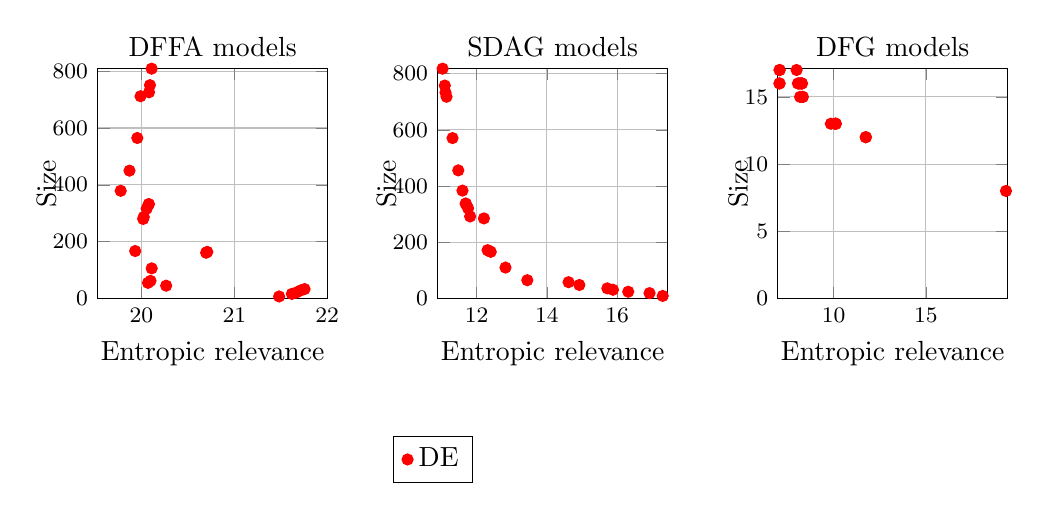
\begin{tikzpicture}
\begin{groupplot}
[group style={group size=3 by 1, vertical sep=1.6cm, horizontal sep=1.4cm}, % Adjust the spacing between plots
xlabel={Entropic relevance}, ylabel={Size}, % Shared labels
tick label style={font=ootnotesize},
legend style={at={(-1.5,-1.22)}, anchor=north, legend columns=3, /tikz/every even column/.append }]
\nextgroupplot[
width=45mm, % Adjusted width
height=45mm, % Adjusted height
xmin=19.529258260538175, % Adjusted x-axis minimum
xmax=22.003119952482088, % Adjusted x-axis maximum
ymin=0, % Adjusted y-axis minimum
ymax=809.0875, % Adjusted y-axis maximum
xlabel={Entropic relevance},
ylabel={Size},
grid=both, % Added grid lines
title={DFFA models},
ylabel style={yshift=-8pt},
title style={yshift=-5pt},
tick label style={font=\footnotesize},
legend style={at={(-1.5,-0.6)}, anchor=north, legend columns=0},  % Adjusted legend position
]
\addplot [scatter, only marks, point meta=explicit symbolic, scatter/classes={
DE={mark=*,red}
},
] table [meta=label] {
	x           y     label
20.10955349994781  809.0  DE
20.056092603482487  316.0  DE
19.871189350403856  450.0  DE
20.708804528594353  164.0  DE
19.77646406130448  379.0  DE
19.95532700514129  565.0  DE
20.09743342508026  62.0  DE
20.081384703759277  726.0  DE
19.990141978233144  712.0  DE
20.091526570159857  751.0  DE
20.11007812232027  106.0  DE
20.02473554671101  287.0  DE
19.932594891887796  167.0  DE
20.078943319967724  332.0  DE
20.078943319967724  332.0  DE
20.696182274591074  161.0  DE
21.48192014465738  7.0  DE
20.01850326165295  280.0  DE
21.619025170811838  16.0  DE
21.666860263882498  21.0  DE
20.26594031665143  45.0  DE
21.712254253084634  28.0  DE
20.070309763886055  55.0  DE
21.755914151715782  33.0  DE
};
\nextgroupplot[
width=45mm, % Adjusted width
height=45mm, % Adjusted height
xmin=10.898172348046355, % Adjusted x-axis minimum
xmax=17.432011746610545, % Adjusted x-axis maximum
ymin=0, % Adjusted y-axis minimum
ymax=818.1125, % Adjusted y-axis maximum
xlabel={Entropic relevance},
ylabel={Size},
grid=both, % Added grid lines
title={SDAG models},
ylabel style={yshift=-8pt},
title style={yshift=-5pt},
tick label style={font=\footnotesize},
legend style={at={(-1.5,-0.6)}, anchor=north, legend columns=0},  % Adjusted legend position
]
\addplot [scatter, only marks, point meta=explicit symbolic, scatter/classes={
DE={mark=*,red}
},
] table [meta=label] {
	x           y     label
11.036123896755802  818.0  DE
11.7603585500143  321.0  DE
11.481219240779984  456.0  DE
12.35828652166278  169.0  DE
11.600719850528959  384.0  DE
11.317849338869953  571.0  DE
13.444408573552549  65.0  DE
11.119352558288645  733.0  DE
11.147918459893335  718.0  DE
11.098374367662311  758.0  DE
12.823675911810254  110.0  DE
11.818473980391188  292.0  DE
12.314555378089409  172.0  DE
11.692976878911791  338.0  DE
11.695700667595617  337.0  DE
12.404663699247722  166.0  DE
17.294060197901096  9.0  DE
12.210131977581222  285.0  DE
16.919374994019194  19.0  DE
16.31385184932588  24.0  DE
14.924144335784348  48.0  DE
15.879225690761832  31.0  DE
14.617099368643675  58.0  DE
15.71956450296964  36.0  DE
};
\nextgroupplot[
width=45mm, % Adjusted width
height=45mm, % Adjusted height
xmin=6.9767896418585105, % Adjusted x-axis minimum
xmax=19.42891877088956, % Adjusted x-axis maximum
ymin=0, % Adjusted y-axis minimum
ymax=17.1, % Adjusted y-axis maximum
xlabel={Entropic relevance},
ylabel={Size},
grid=both, % Added grid lines
title={DFG models},
ylabel style={yshift=-8pt},
title style={yshift=-5pt},
tick label style={font=\footnotesize},
legend style={at={(-1.5,-0.6)}, anchor=north, legend columns=0},  % Adjusted legend position
]
\addplot [scatter, only marks, point meta=explicit symbolic, scatter/classes={
DE={mark=*,red}
},
] table [meta=label] {
	x           y     label
7.995939987033551  17.0  DE
8.066221914899987  16.0  DE
8.107337162106173  16.0  DE
8.1844741203791  15.0  DE
8.15913810968429  16.0  DE
7.0651034347934285  16.0  DE
9.851433492366969  13.0  DE
7.072190058170718  17.0  DE
7.075091548626624  16.0  DE
7.077687053162569  17.0  DE
8.293821437858991  15.0  DE
8.247918942852225  16.0  DE
8.311879177957115  15.0  DE
8.263551500020418  16.0  DE
8.270548142567073  16.0  DE
8.334324065411773  15.0  DE
19.34060497795464  8.0  DE
8.289037608143794  16.0  DE
11.735947626442124  12.0  DE
11.755618362776016  12.0  DE
10.091462696217874  13.0  DE
10.101626622184881  13.0  DE
10.111338668189868  13.0  DE
10.120637310128991  13.0  DE
};
\legend{{DE}};

\end{groupplot}
\end{tikzpicture}
\vspace{-2.75mm}
\caption{Size and entropic relevance of discovered DFFAs}
\end{center}
\end{figure}
\begin{table}[htbp]
\vspace{-11mm}
\caption{DCI comparision(\%)}\label{tbl:3}
\centering % used for centering table
\setlength{\tabcolsep}{1pt} % Adjust this value to 
\fontsize{7}{9}\selectfont
\begin{tabular}{|l|c|}
\hline %insert double horizontal lines
\,Event log &DE\\
\hline %insert double horizontal lines
BPI\_2013.xes&31.56\\
\hline %inserts single line
\end{tabular}
\vspace{-2.75mm}
\end{table}
Tables 2 and 3 summarize the analysis of the diversity of the models and the global Pareto front (dominance count), respectively. Figure 1 shows the characteristics of the Pareto-optimal models discovered from the
BPI\_2013.xes by the selected algorithm.
\begin{table}[htbp]
\vspace{-1mm}
\caption{Pareto dominance count comparision}\label{tbl:2}
\centering % used for centering table
\setlength{\tabcolsep}{1pt} % Adjust this value to 
\fontsize{7}{9}\selectfont
\begin{tabular}{|l|c|c|}
\hline %insert double horizontal lines
\,Event log &DE&Total\\
\hline %insert double horizontal lines
BPI\_2013.xes&100.00&24 100.00\%\\
\hline %inserts single line
\end{tabular}
\vspace{-3.75mm}
\end{table}

\begin{table}[htbp]
\vspace{-1mm}
\caption{Execution time comparision (iteration per second}\label{tbl:4}
\centering % used for centering table
\setlength{\tabcolsep}{1pt} % Adjust this value to 
\fontsize{7}{9}\selectfont
\begin{tabular}{|l|c|
}
\hline %insert double horizontal lines
\,Event log &DE\\
\hline %insert double horizontal lines
BPI\_2013.xes&2.14\\
\hline %inserts single line
\end{tabular}
\vspace{-3.75mm}
\end{table}

\section{Online Resources}
Updated algorithms are publicly available via the following links.
\begin{itemize}
\item
\href{https://github.com/HzhianUnimelb/BPM_ProcessDiscovery_Optimization}{Process Discovery Optimization}.
\end{itemize}
The following link refers to the details of candidate models generated by algorithms.
\begin{itemize}
\item
\href{C:/Users/hzhian/eclipse-workspace/processICPM/20250730_152959}{Candidate pareto frontier models}.
\end{itemize}
\section{References}
[1].  Li, M., Yang, S., Liu, X.: Diversity comparison of Pareto front approximations in many-objective
optimiation. IEEE Trans. Cybern.44(12), 2568–2584 (2014)
\section{Appendix}
Tables 5 lists the quality parameters of candidate models by the selected algorithms.\begin{table}[htbp]
\vspace{-5mm}
\caption{Details of candidates models}\vspace{+1mm}
\label{tbl:5}
\centering % used for centering table
\setlength{\tabcolsep}{1pt} % Adjust this value to 
\fontsize{7}{9}\selectfont
\begin{tabular}{|l|c|c|}
\hline
\,Method & size & Entropic relevance \\
\hline %insert double horizontal lines 
DE&818.0&11.036\\\hline %insert double horizontal lines 
DE&321.0&11.760\\\hline %insert double horizontal lines 
DE&456.0&11.481\\\hline %insert double horizontal lines 
DE&169.0&12.358\\\hline %insert double horizontal lines 
DE&384.0&11.601\\\hline %insert double horizontal lines 
DE&571.0&11.318\\\hline %insert double horizontal lines 
DE&65.0&13.444\\\hline %insert double horizontal lines 
DE&733.0&11.119\\\hline %insert double horizontal lines 
DE&718.0&11.148\\\hline %insert double horizontal lines 
DE&758.0&11.098\\\hline %insert double horizontal lines 
DE&110.0&12.824\\\hline %insert double horizontal lines 
DE&292.0&11.818\\\hline %insert double horizontal lines 
DE&172.0&12.315\\\hline %insert double horizontal lines 
DE&338.0&11.693\\\hline %insert double horizontal lines 
DE&337.0&11.696\\\hline %insert double horizontal lines 
DE&166.0&12.405\\\hline %insert double horizontal lines 
DE&9.0&17.294\\\hline %insert double horizontal lines 
DE&285.0&12.210\\\hline %insert double horizontal lines 
DE&19.0&16.919\\\hline %insert double horizontal lines 
DE&24.0&16.314\\\hline %insert double horizontal lines 
DE&48.0&14.924\\\hline %insert double horizontal lines 
DE&31.0&15.879\\\hline %insert double horizontal lines 
DE&58.0&14.617\\\hline %insert double horizontal lines 
DE&36.0&15.720\\\hline %insert double horizontal lines 
\end{tabular}
\vspace{-3.75mm}
\end{table}

\end{document}